\documentclass{article}
\usepackage{blindtext}
\usepackage[paperheight=11in,paperwidth=8.5in,margin=1in]{geometry}
\usepackage[utf8]{inputenc}
\usepackage[english]{babel}
\usepackage{graphicx}
\usepackage{csquotes}
\usepackage[backend=biber,style=alphabetic,maxbibnames=999]{biblatex}
\usepackage[colorlinks]{hyperref}

\pagenumbering{gobble}

\newcommand{\fig}[1]{\hyperref[fig:#1]{Figure~\ref*{fig:#1}}}

\addbibresource{references.bib}

\title{
Falling with Style: Factoring up to 255 ``with'' a Quantum Computer
}
\author{Craig Gidney}

\date{April 1, 2025}

\begin{document}

\maketitle

\begin{abstract}
In this paper, I explain how I factored all numbers up to 255 using Shor's algorithm on a real quantum computer.
I performed \emph{exactly} the classical preprocessing specified by Shor's algorithm,
\emph{exactly} the quantum circuit requested by Shor's algorithm,
and \emph{exactly} the post-processing specified by Shor's algorithm.
In total this involved sampling the quantum computer 121 times.
This slightly underperformed the 120 samples used when sampling from a random number generator instead.
\end{abstract}

\section{Intro}

Historically, most papers that claimed they ``ran Shor's algorithm'' didn't run Shor's algorithm.
It's unfortunately common to run circuits \emph{inspired by} Shor's algorithm, but with key pieces replaced by trivial pieces~\cite{Vandersypen2001,Lanyon2007,Lu2007,MartnLpez2012,lucero2012}.
The issue is that, in the large shenanigans limit, all quantum factoring circuits are trivial~\cite{Smolin2013}.
In this paper, I don't make that mistake.
I run Shor's algorithm exactly as it was supposed to be run: with comically underoptimized circuits.
Nevertheless, the circuits work.
They quickly result in factors being produced.
This naturally raises the question: ``What's the catch?''.
Because of course there's a catch.

The key insight here is that, for small numbers, Shor's algorithm is surprisingly resilient to noise.
It's so resilient that, even if you replace the quantum computer with a random number generator, the algorithm still succeeds with high probability!
This is serendipitous because, when a quantum computer is given a circuit that's way too large, the output approximates a random number generator.
In other words, for small numbers, Shor's algorithm succeeds quickly \emph{regardless of how well your quantum computer works}.

Factoring in this way reminds me of a scene from Toy Story.
In the scene, Buzz Lightyear (see \fig{results}) attempts to fly.
He doesn't actually fly but, due a humorous series of coincidences, appears to.
Another toy, Woody, complains that Buzz was just ``falling with style''.
The rest of the toys don't care.
Similarly, in this paper, I will appear to succeed at factoring by falling with style.


\section{Methods}

I wrote python code (available at \href{https://github.com/strilanc/falling-with-style}{github.com/strilanc/falling-with-style}) that produces a quantum circuit that performs the quantum part of Shor's algorithm.
The generated circuit performs a modular exponentiation and then a frequency basis measurement.
I implemented the modular exponentiation by decomposing it into modular multiplications, then decomposing those into fused modular multiply-adds, then decomposing those into modular additions, then decomposing those into 2s-complement additions / subtractions / comparisons, then decomposing those into textbook CCX/CX/X gates~\cite{cuccaro2004}.
For the frequency basis measurement I wanted to use qubit recycling~\cite{Mosca1999} to save space, but the quantum computer I chose (\texttt{IBM\_SHERBROOKE}) doesn't support classical feedback.
So I simply performed the textbook quantum Fourier transform circuit followed by computational basis measurement.
The textbook gates were converted into physical gates by Qiskit's automatic transpilation tools.

I was initially worried that IBM's quantum service would reject my factoring circuits, because IBM's documentation only guarantees circuits will fit into hardware memory limits if they have fewer than ten thousand two-qubit gates~\cite{joblimits}.
My circuits are much larger than this.
For example, after transpilation, my circuit for factoring 15 weighs in at 44405 two-qubit gates.
And my circuit for factoring 253 weighs in at 245750 two-qubit gates.
Amazingly, despite the fact that they vastly exceed the allowed size, the system accepted these ridiculous circuits.

When I submitted the circuits, the two qubit gate error rate reported by the system was 1.41\%.
With this error rate, it would be difficult to extract signal from a computation that used a thousand gates nevermind a hundred thousand.
So I was confident that my circuits would sufficiently randomize the output, achieving the goal of factoring by falling with style.

To insert a bit of competition, I decided to run my circuits not just against a real quantum computer but also against a simulated noiseless quantum computer and against a random number generator.
I wanted to see how the real machine compared to these two extremes.
To compare them, I counted how many times the quantum part of Shor's algorithm was executed (how many quantum samples were collected).
Fewer samples is better, because it's more efficient.

Before showing the results, to ensure the reader understands what it means for a quantum sample to occur, I'll quickly review the classical and quantum steps of Shor's algorithm.
Before talking to a quantum computer, Shor's algorithm performs some classical preprocessing.
First, it checks if $n$ (the number to factor) is even, because even numbers would cause trouble later.
If so, it succeeds by returning the factor 2.
Second, it checks if $n$ is prime.
Prime numbers can't be factored, so in this case the method returns an error saying no factor exists.
Third, the algorithm picks a random number $g$ between $2$ and $n-2$, and computes the greatest common divisor (gcd) of $g$ and $n$.
If $\gcd(g, n) \neq 1$, then it happens to be a factor of $n$ and so is returned as the result.
Fourth, it's finally time to actually use the quantum computer (whether it be real, simulated, or replaced by a random number generator).
This is the expensive step, and the step that I'm counting in order to compare the different samplers.
A quantum circuit based on $g$ and $n$ is generated, and executed, producing a sample $m$.
Fifth, Shor's algorithm classically computes the fraction that's closest to $m/4^{\lceil \log_2(n) \rceil}$, limiting the fraction's denominator $d$ to be at most $n$.
Sixth, a candidate factor is generated by computing $\gcd(n, 1 + g^{\lfloor d / 2 \rfloor} \bmod n)$.
If the candidate is actually a factor of $n$, it's returned as the answer.
Otherwise the algorithm restarts.

As an example, let's consider factoring 253 into $11 \times 23$.
253 isn't even or prime, so the algorithm advances to picking a random value $g$ in $[2, 251]$.
32 of the 249 possible values of $g$ share a factor with 253, caught by the gcd check, so there's a $12.9\%$ chance the algorithm terminates due to $g$ before collecting a quantum sample $m$.
Of the 14221312 possible pairs $(g, m)$, 1752324 ($12.3\%$) of them result in the postprocessing producing a factor.
Accounting for both these ways of succeeding, replacing the quantum computer with a random number generator results in nearly a 25\% chance of success per quantum sample.
So the expected number of shots to factor 253 is a bit more than 4.
With a noiseless quantum computer, the expected number of shots to factor 253 would instead be roughly 2.5.


\section{Results}

The experimental results are shown in \fig{results}.
Factoring all numbers up to 255 resulted in the simulated noiseless quantum computer being sampled 94 times, the random number generator being sampled 120 times, and the real quantum computer being sampled 121 times.

Not surprisingly, the simulated noiseless quantum computer was the most sample efficient.
However, because 255 is such a small number, the advantage isn't large.
There were even times where, if I had stopped the experiment, the noiseless simulator would have lost to the random number generator.
For large numbers, Shor's algorithm has an enormous advantage over random guessing.
For these small numbers, the advantage is more tenuous.

\begin{figure}
    \centering
    \resizebox{\linewidth}{!}{
    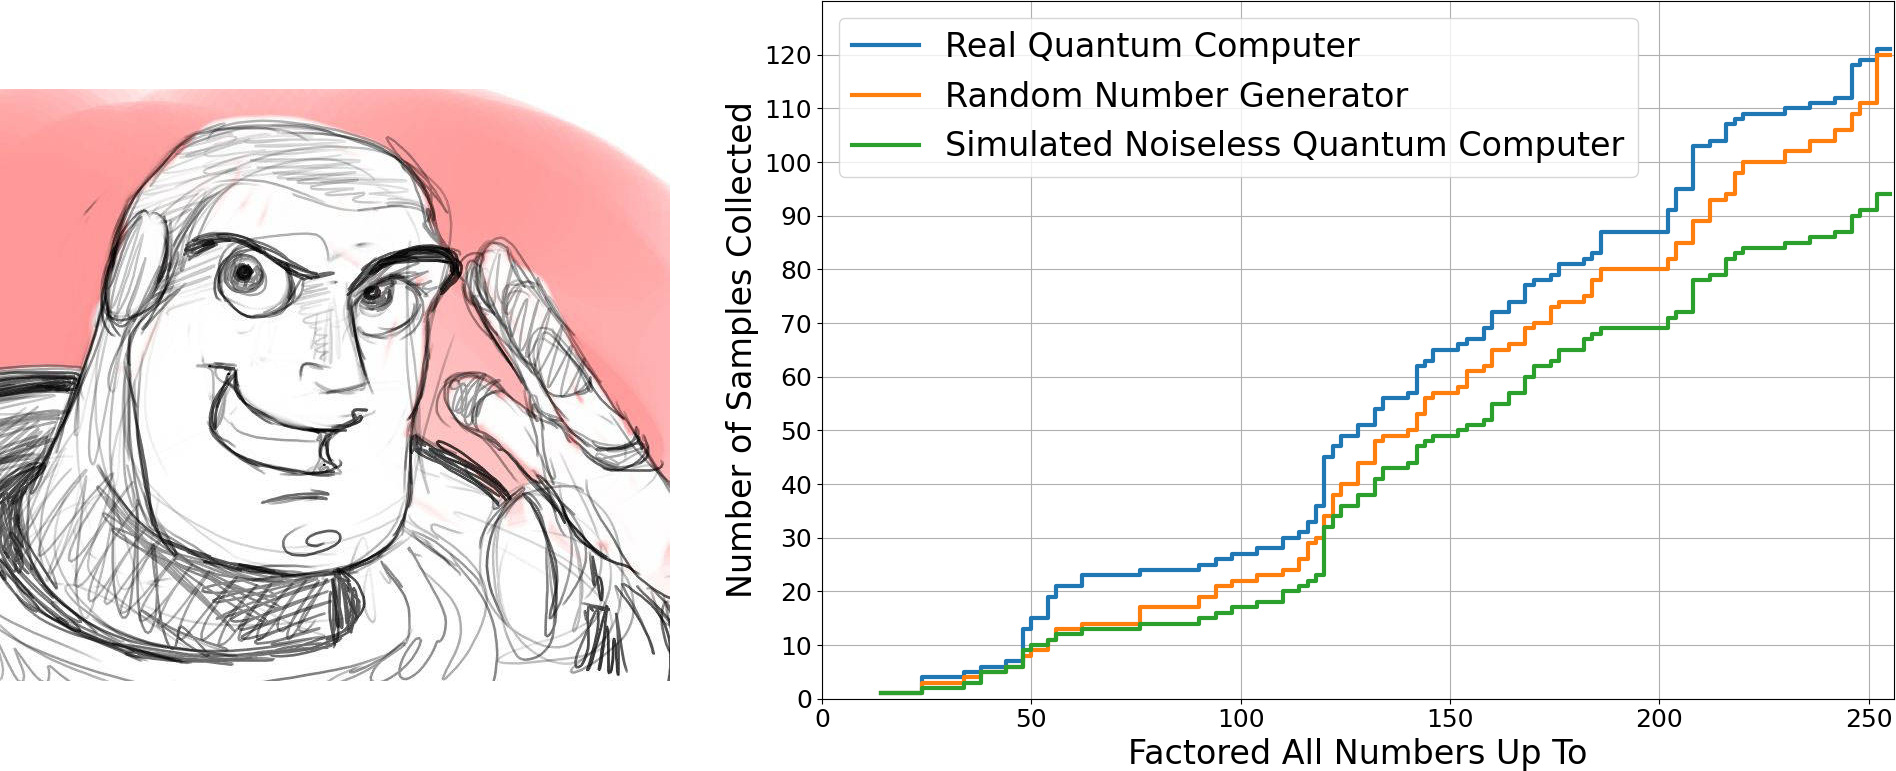
\includegraphics{results.png}
    }
    \caption{
        Left: A creative commons sketch of Buzz Lightyear from Deviant Art~\cite{buzzsketch}.
        Right: comparing the sample efficiency of factoring all numbers up to 255 with a variety of sampling devices.
    }
    \label{fig:results}
\end{figure}

Humorously, the real quantum computer does slightly worse than the random number generator.
Following the plot from left to right: the real quantum computer has a bad start, then manages to keep pace, and even starts to gain near the end, but falls just short in a photo finish~\cite{xkcdsports}.
I could repeat the experiment many times to verify this was just random bad luck, but IBM only provides 10 free minutes of quantum computer time per month and I consumed half of that running the experiment once.
Also, this way's funnier.


\section{Conclusion}

To my knowledge, no one has cheated at factoring in this way before.
Given the shenanigans pulled by past factoring experiments, that's remarkable.

Ultimately, the key to factoring small numbers isn't making the quantum computer ``work well''.
That's the key to factoring \emph{large} numbers.
For small numbers it's sufficient to strap a hopelessly oversized circuit to the quantum processor, light the fuse, and shout ``To infinity and beyond!''.

\printbibliography

\end{document}
